\documentclass[border=3mm]{standalone}
\usepackage{tikz}

\begin{document}
    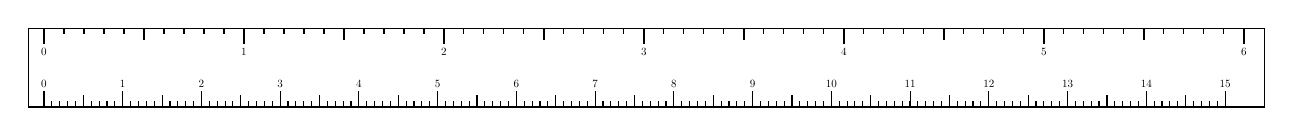
\begin{tikzpicture}
        \draw (-0.2,0) rectangle (15.5,1);
        %% lower divisions
        \foreach \x in {0,1,...,15}{
            \draw (\x,0) -- (\x,0.2)node[above,scale=0.4]{\x};
        }
        \foreach \x in {0.1,0.2,...,14.9}{
            \draw (\x,0) -- (\x,0.075);
        }
        \foreach \x in {0.5,1,...,14.5}{
            \draw (\x,0) -- (\x,0.15);
        }
        % Upper divisions
        \foreach \x in {0,1,...,6}{
            \draw (\x in,1) -- (\x in,0.8)node[below,scale=0.4]{\x};
        }
        \foreach \x in {0.1,0.2,...,5.9}{
            \draw (\x in,1) -- (\x in,0.925);
        }
        \foreach \x in {0.5,1,...,5.5}{
            \draw (\x in,1) -- (\x in,0.85);
        }
    \end{tikzpicture}
\end{document}
